\documentclass[11pt]{article}
\usepackage[margin=1in]{geometry}
\usepackage{graphicx}
\usepackage{booktabs}
\usepackage{amsmath}
\usepackage{xcolor}
\usepackage{caption}
\usepackage{float}
\usepackage[colorlinks=true,linkcolor=black,citecolor=blue,urlcolor=blue]{hyperref}
\captionsetup{font=small,labelfont=bf}
\graphicspath{{figs/}}

\definecolor{best}{HTML}{2E7D3E}
\newcommand{\best}[1]{\textcolor{best}{\textbf{#1}}}

\title{\vspace{-1.5em}\textbf{Procedure Step Recognition on Egocentric Assembly Video:\\
An Architecture Progression from VideoMAE+ASFormer to Fusion+DiffAct,\\ with a SAM3 Enrichment Layer}}
\author{Ego-centric PSR Project \\ \small IndustReal \& MECCANO}
\date{}

\begin{document}
\maketitle
\vspace{-2em}

\begin{abstract}
\noindent
We study \emph{procedure step recognition} (PSR) on egocentric assembly video: given a first-person
video of a construction task, output a dense timeline ``from $t_0$ to $t_1$ $\rightarrow$ \textit{part}
(correct\,/\,incorrect\,/\,remove).'' We frame PSR as temporal action segmentation with a two-stage recipe:
a \emph{frozen} video backbone produces per-clip features and only a lightweight segmentation head is trained.
Starting from a VideoMAEv2\nobreakdash-Huge $+$ ASFormer baseline, we present a controlled progression in which
\emph{every architecture change yields a measurable improvement}: procedure-aware Viterbi decoding, a stronger
SSv2\nobreakdash-pretrained giant backbone, a diffusion segmentation head (DiffAct), and a two-encoder feature
fusion (VideoMAEv2 $+$ InternVideo2). The final model, \textbf{v4 = Fusion $+$ DiffAct}, reaches
\best{F1@50 $=70.1$} on the IndustReal test split---a $+13.8$ point gain over the baseline and the first result
above $70$. We further build a causal real-time variant, confirm the recipe generalizes to a second dataset
(MECCANO), and analyze the \emph{correctness} sub-problem, which we show to be data-limited rather than
method-limited. Finally, we add an inference-time \textbf{SAM3 enrichment layer} that augments the timeline with
per-step object masks and a component inventory. We report that promptable foundation models (LocateAnything,
SAM3) reliably \emph{localize} parts but do not \emph{judge} correctness, and we position SAM3 as an output-enrichment
component rather than a correctness classifier.
\end{abstract}

\section{Introduction}
Egocentric video of manual assembly is a natural testbed for fine-grained procedure understanding: the camera
sees the worker's hands and the evolving object state, and errors are induced deliberately. We target
\textbf{IndustReal}~\cite{industreal}, a dataset of $84$ recordings of a toy construction (STEMFIE) split
$36/16/32$ into train/val/test, annotated with procedure-step completions including \emph{incorrectly installed}
and \emph{removed} events. Our goal is a system that emits, for a full recording, a dense per-step timeline with
a correctness verdict per step.

We adopt the classic two-stage temporal action segmentation (TAS) recipe~\cite{mstcn,asformer}: a large,
\emph{frozen} self-supervised video backbone provides per-clip features, and a comparatively small head is trained
on top. This keeps training cheap and lets us treat the backbone and head as independent design axes. The
contributions of this report are:
\begin{itemize}
  \item A \textbf{controlled architecture progression} in which each change---decoding, backbone, head, and
  feature fusion---improves segmentation quality, culminating in \best{v4 (Fusion $+$ DiffAct), F1@50 $=70.1$}
  (Fig.~\ref{fig:prog}, Table~\ref{tab:score}).
  \item A \textbf{causal real-time} variant and a \textbf{cross-dataset} confirmation on MECCANO~\cite{meccano}.
  \item An analysis showing the \textbf{correctness} problem is \emph{data-limited}, not method-limited.
  \item A \textbf{SAM3 enrichment layer}~\cite{sam3} that adds per-step masks and a component inventory at inference,
  together with a negative but useful result: promptable models locate but do not judge correctness.
\end{itemize}

\section{Background and Related Work}
\textbf{Temporal action segmentation.} MS-TCN~\cite{mstcn} popularized multi-stage temporal convolutions for
per-frame action labeling; ASFormer~\cite{asformer} introduced a transformer encoder--decoder for the same task.
DiffAct~\cite{diffact} recasts segmentation as an iterative denoising (diffusion) process and yields sharp
boundaries. \textbf{Video backbones.} VideoMAEv2~\cite{videomae} is a masked-autoencoder video transformer;
we use its Huge (K710) and giant (SSv2) variants. InternVideo2~\cite{internvideo2} is a strong appearance/semantic
video encoder that we fuse with VideoMAEv2. \textbf{Streaming.} MiniROAD~\cite{miniroad} and TeSTra~\cite{testra}
inform our causal head design. \textbf{Promptable foundation models.} SAM~\cite{sam} and SAM2~\cite{sam2}
established promptable segmentation; SAM3~\cite{sam3} adds open-vocabulary \emph{concept} segmentation and video
tracking. LocateAnything~\cite{locateanything} (built on Qwen2.5~\cite{qwen25}) is a grounding VLM that returns
boxes/points. We evaluate the latter two for a correctness/enrichment role.

\section{Method: the two-stage pipeline}
For a recording we sample $16$-frame clips at a fixed stride and pass each clip through the frozen backbone to
obtain a feature $x_t \in \mathbb{R}^{D}$; the sequence $\{x_t\}$ is fed to the trained head, which predicts a
per-clip \textbf{step} label ($10$ parts $+$ background $=11$ classes). Consecutive equal labels are merged into
segments, giving the ``which part / when'' timeline. A parallel \textbf{type} head predicts
correct\,/\,incorrect\,/\,remove and is pooled per segment. Metrics follow the MS-TCN protocol~\cite{mstcn}:
frame accuracy, segmental edit score, and F1 at IoU thresholds $\{10,25,50\}\%$.

\section{Architecture progression}
\label{sec:prog}
We now walk through the design changes; each is evaluated on the IndustReal test split (Table~\ref{tab:score},
Fig.~\ref{fig:prog}).

\paragraph{v1 --- VideoMAEv2-Huge $+$ ASFormer (baseline).}
A distilled Huge (K710, $1280$-d) backbone with an ASFormer head establishes the baseline at F1@50 $=56.3$.

\paragraph{$+$ Viterbi decoding.}
Replacing raw arg-max with a procedure-aware Viterbi smoothing over the head's log-probabilities removes spurious
short segments and lifts the boundary metrics substantially: F1@50 $62.2$ ($+5.9$), edit $68.8\!\to\!74.2$.

\paragraph{v2 --- SSv2-giant features.}
Swapping the backbone for a VideoMAEv2 \emph{giant} model fine-tuned on Something-Something-v2 ($1408$-d), with
no center crop and a finer stride, improves temporal grounding: F1@50 $66.5$ ($+4.3$).

\paragraph{v2 --- DiffAct head.}
Replacing ASFormer with the diffusion head DiffAct~\cite{diffact} on the same SSv2 features yields the sharpest
boundaries so far: F1@50 $68.9$, edit $79.6$.

\paragraph{Fusion --- adding InternVideo2.}
Motivated by the correctness sub-problem, we fuse a motion-centric encoder (giant SSv2, $1408$-d) with an
appearance/semantic encoder (InternVideo2-B14, $768$-d) by $\ell_2$-normalizing each stream and concatenating to a
$2176$-d representation. With an ASFormer head this matches DiffAct on segmentation (F1@50 $68.2$) while, crucially,
being the \emph{only} configuration to produce non-zero fault detection (Sec.~\ref{sec:correct}).

\paragraph{v4 --- Fusion $+$ DiffAct (best).}
The two wins are \emph{orthogonal}: fusion improves the \emph{features}, DiffAct improves the \emph{head}. Combining
them---feeding the $2176$-d fusion features to DiffAct---gives our best model,
\best{Acc $74.9$ / Edit $79.5$ / F1@50 $70.1$}, the first result above $70$ and $+13.8$ over the baseline
(Fig.~\ref{fig:v4}).

\begin{figure}[H]
\centering
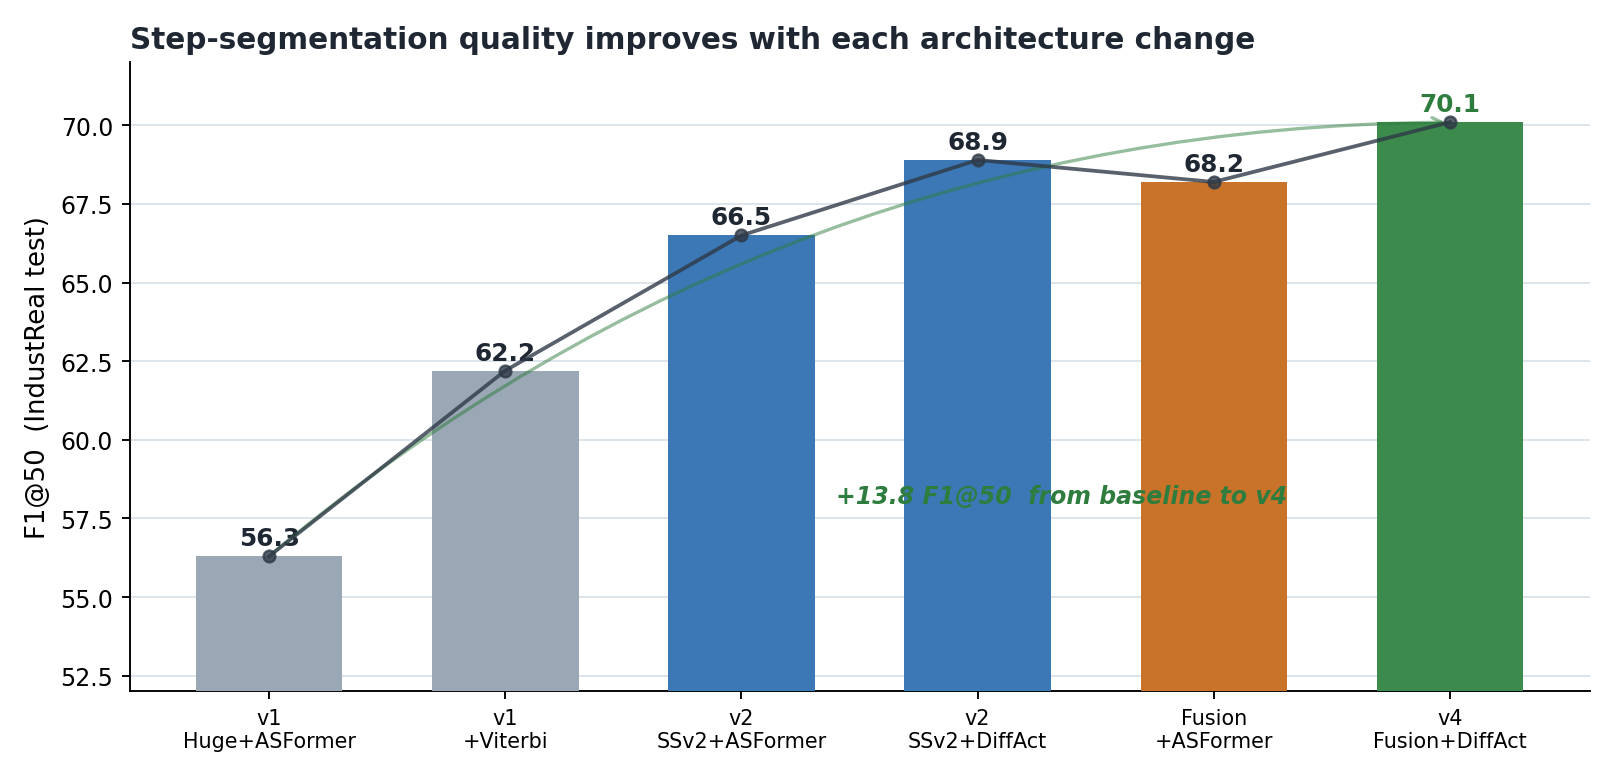
\includegraphics[width=0.92\linewidth]{fig_f1_progression.png}
\caption{Step-segmentation F1@50 on the IndustReal test split improves at each architecture change,
from the v1 baseline ($56.3$) to \best{v4 ($70.1$)}.}
\label{fig:prog}
\end{figure}

\begin{table}[H]
\centering
\caption{Offline step-segmentation scorecard (IndustReal test, $32$ recordings). Higher is better.
\best{v4} is the best model.}
\label{tab:score}
\small
\begin{tabular}{lccccc}
\toprule
Configuration & Acc & Edit & F1@10 & F1@25 & F1@50 \\
\midrule
v1\ \ Huge-K710 $+$ ASFormer (baseline) & 73.3 & 68.8 & 72.9 & 68.6 & 56.3 \\
v1\ \ $+$ Viterbi                        & 73.4 & 74.2 & 78.6 & 73.9 & 62.2 \\
v2\ \ SSv2-giant $+$ ASFormer $+$ Viterbi & 74.0 & 77.3 & 80.0 & 76.5 & 66.5 \\
v2\ \ SSv2-giant $+$ DiffAct              & 74.4 & 79.6 & 81.1 & 77.6 & 68.9 \\
Fusion (giant$+$IV2-B14) $+$ ASFormer $+$ Viterbi & 75.7 & 77.6 & 79.0 & 75.8 & 68.2 \\
\midrule
\best{v4\ \ Fusion $+$ DiffAct \ (best)} & \best{74.9} & \best{79.5} & \best{83.1} & \best{79.1} & \best{70.1} \\
\bottomrule
\end{tabular}
\end{table}

\begin{figure}[H]
\centering
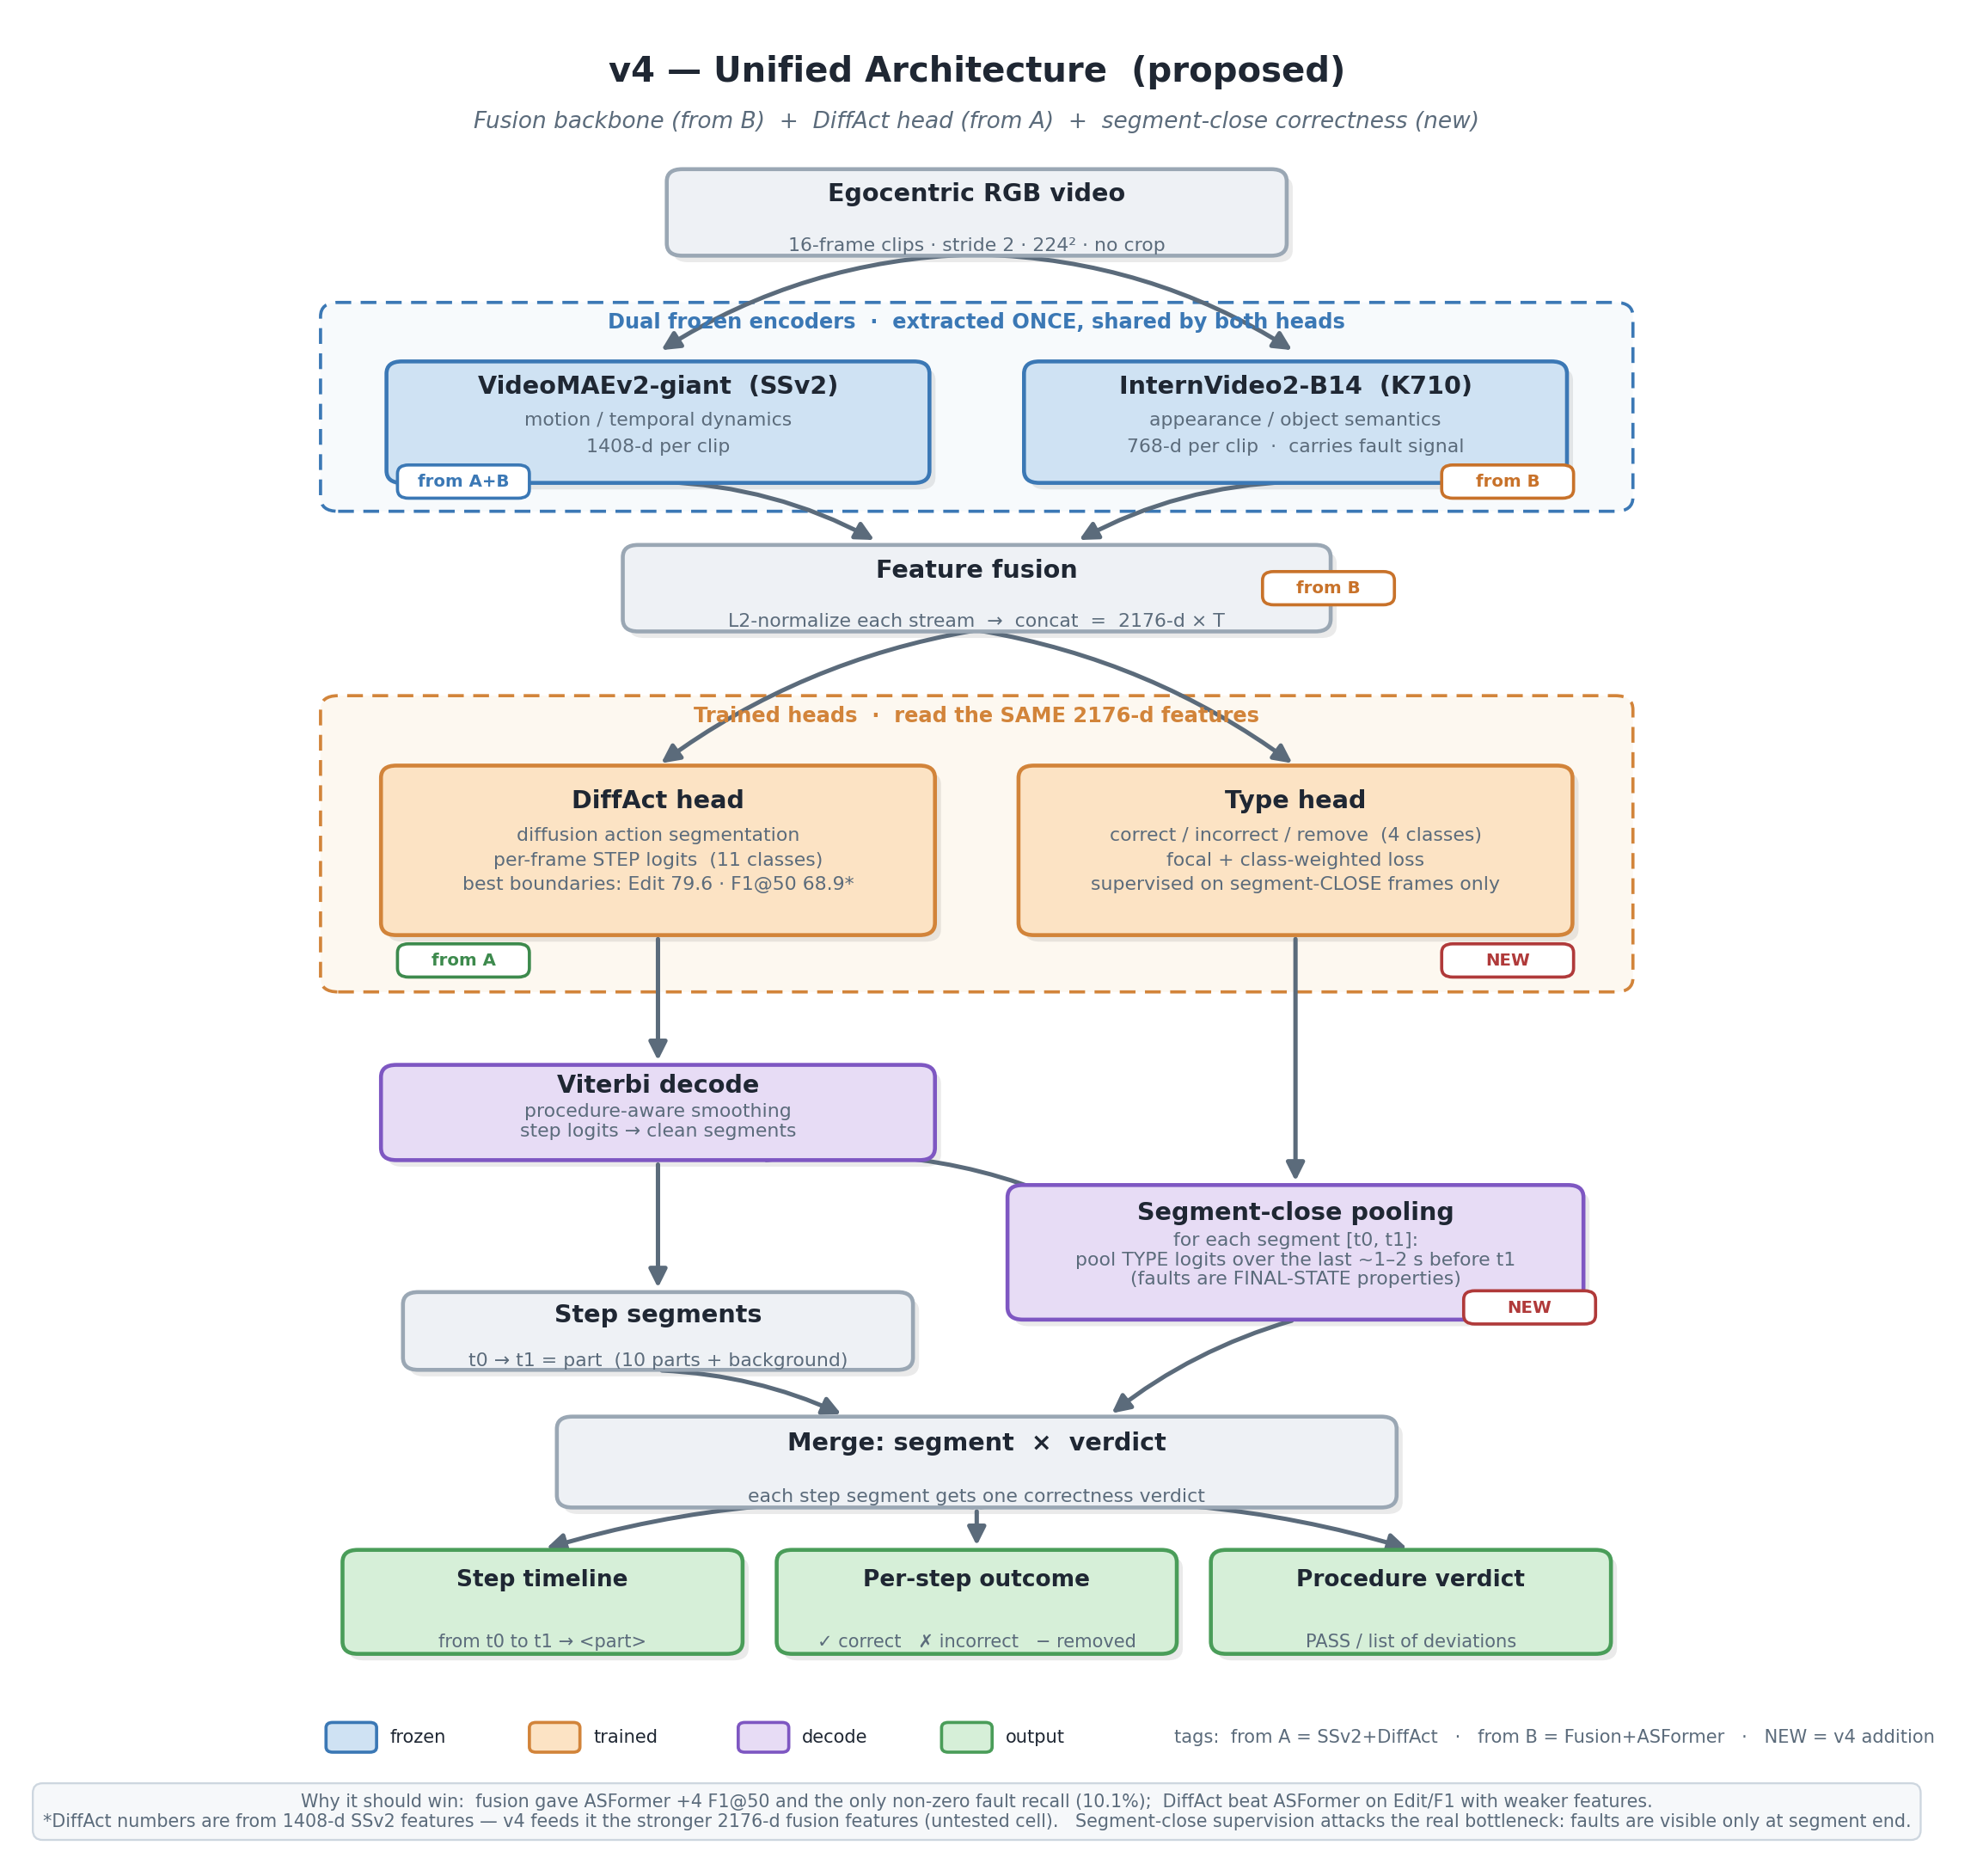
\includegraphics[width=0.62\linewidth]{architecture_v4.png}
\caption{The v4 unified architecture: dual frozen encoders (VideoMAEv2-giant $+$ InternVideo2-B14) $\rightarrow$
$2176$-d fusion features $\rightarrow$ DiffAct step head; a parallel type head predicts correctness. Provenance
tags mark which component each part inherits.}
\label{fig:v4}
\end{figure}

\paragraph{Real-time streaming (v3).}
For online use we build a fully causal variant: a distilled ViT-B backbone over a $16$-frame window ending at $t$,
MiniROAD-style causal GRU heads~\cite{miniroad}, and a fixed-lag online Viterbi that commits frame $t-L$. At
$L{=}16$ ($\approx2.7$\,s latency) it reaches edit $55.3$ / F1@50 $37.4$. A TeSTra head~\cite{testra}
under-performed the GRU ($24.8$ F1@50), consistent with transformers being data-hungry on our $36$-recording
training set.

\paragraph{Cross-dataset (MECCANO).}
Applying the same fusion$+$ASFormer recipe unchanged to MECCANO~\cite{meccano} ($20$ recordings, $18$ step classes)
gives F1@50 $38.0$, confirming the framework generalizes.

\section{The correctness sub-problem}
\label{sec:correct}
Correctness (\emph{was the step done right?}) is markedly harder than segmentation. The type head's
incorrect-install recall is $0\%$ for any VideoMAE-only backbone and rises to \textbf{$10.1\%$} only with the
InternVideo2 fusion---the first non-zero fault detection (Table~\ref{tab:extra}). A larger appearance encoder
(InternVideo2-L14) \emph{regressed} to $0\%$, and on MECCANO recall is also $0\%$. We conclude correctness is
\textbf{data-limited, not method-limited}: with only $\sim$29 labeled incorrect events, encoder capacity is not
the lever---more and sharper error labels are.

\begin{table}[H]
\centering
\caption{Correctness (incorrect-install recall) and real-time streaming summary.}
\label{tab:extra}
\small
\begin{tabular}{lcc}
\toprule
\multicolumn{3}{l}{\textit{Correctness --- type head, IndustReal}} \\
\midrule
Configuration & Incorrect recall & Remove recall \\
Any VideoMAE-only $+$ ASFormer & $0.0\%$ & $\sim$68\% \\
\best{Fusion giant $+$ InternVideo2-B14} & \best{$10.1\%$} & $69.4\%$ \\
Fusion giant $+$ InternVideo2-L14 & $0.0\%$ & --- \\
\midrule
\multicolumn{3}{l}{\textit{Real-time streaming --- IndustReal, causal}} \\
\midrule
Configuration & F1@50 & Latency \\
\best{v3 causal ViT-B $+$ GRU ($L{=}16$)} & \best{$37.4$} & $2.7$\,s \\
v3 TeSTra head ($L{=}16$) & $24.8$ & $2.7$\,s \\
\bottomrule
\end{tabular}
\end{table}

\subsection{Can a promptable foundation model judge correctness?}
We tested two recent models on our hardware (AMD MI210 / ROCm). \textbf{LocateAnything}~\cite{locateanything}
(a $3$B grounding VLM) and \textbf{SAM3}~\cite{sam3} (a $0.9$B promptable segmenter) both reliably
\emph{localize} the STEMFIE parts for coarse categories (wheel, screw, bracket). However, on a part-matched set
of $\sim$57 correct-vs-incorrect installs, neither could \emph{judge} correctness: LocateAnything echoed the
prompt as a referring expression and returned boxes regardless of the true label ($100\%$ recall / $51\%$
precision $=$ chance), and SAM3 segments a part whether or not it is faulty. Both are \emph{locators, not judges};
correctness requires a downstream comparison against a reference, which no perception model supplies.

\section{SAM3 enrichment layer}
Given the above, we use SAM3 not for correctness but to \textbf{enrich the output} at inference
(Fig.~\ref{fig:sam3}). SAM3 produces pixel-accurate instance masks (far sharper than the boxes of the VLM) and
supports video tracking. We wire it on top of the frozen v4 pipeline: for each committed step segment we run SAM3
with the coarse category of the step's part and overlay the resulting masks, and we aggregate a per-recording
\textbf{component inventory}. The result is the same v4 timeline augmented with (i) per-step part masks (the
``where'') and (ii) a component inventory (``what is present''), with \emph{no retraining and identical accuracy}
(Fig.~\ref{fig:enriched}). SAM3 masks and video tracking further enable, as future work, \emph{omission} and
\emph{rework} detection (comparing the inventory to an expected bill-of-materials, and tracking part identities
over time)---signals that are not data-limited because they do not depend on the scarce incorrect labels.

\begin{figure}[H]
\centering
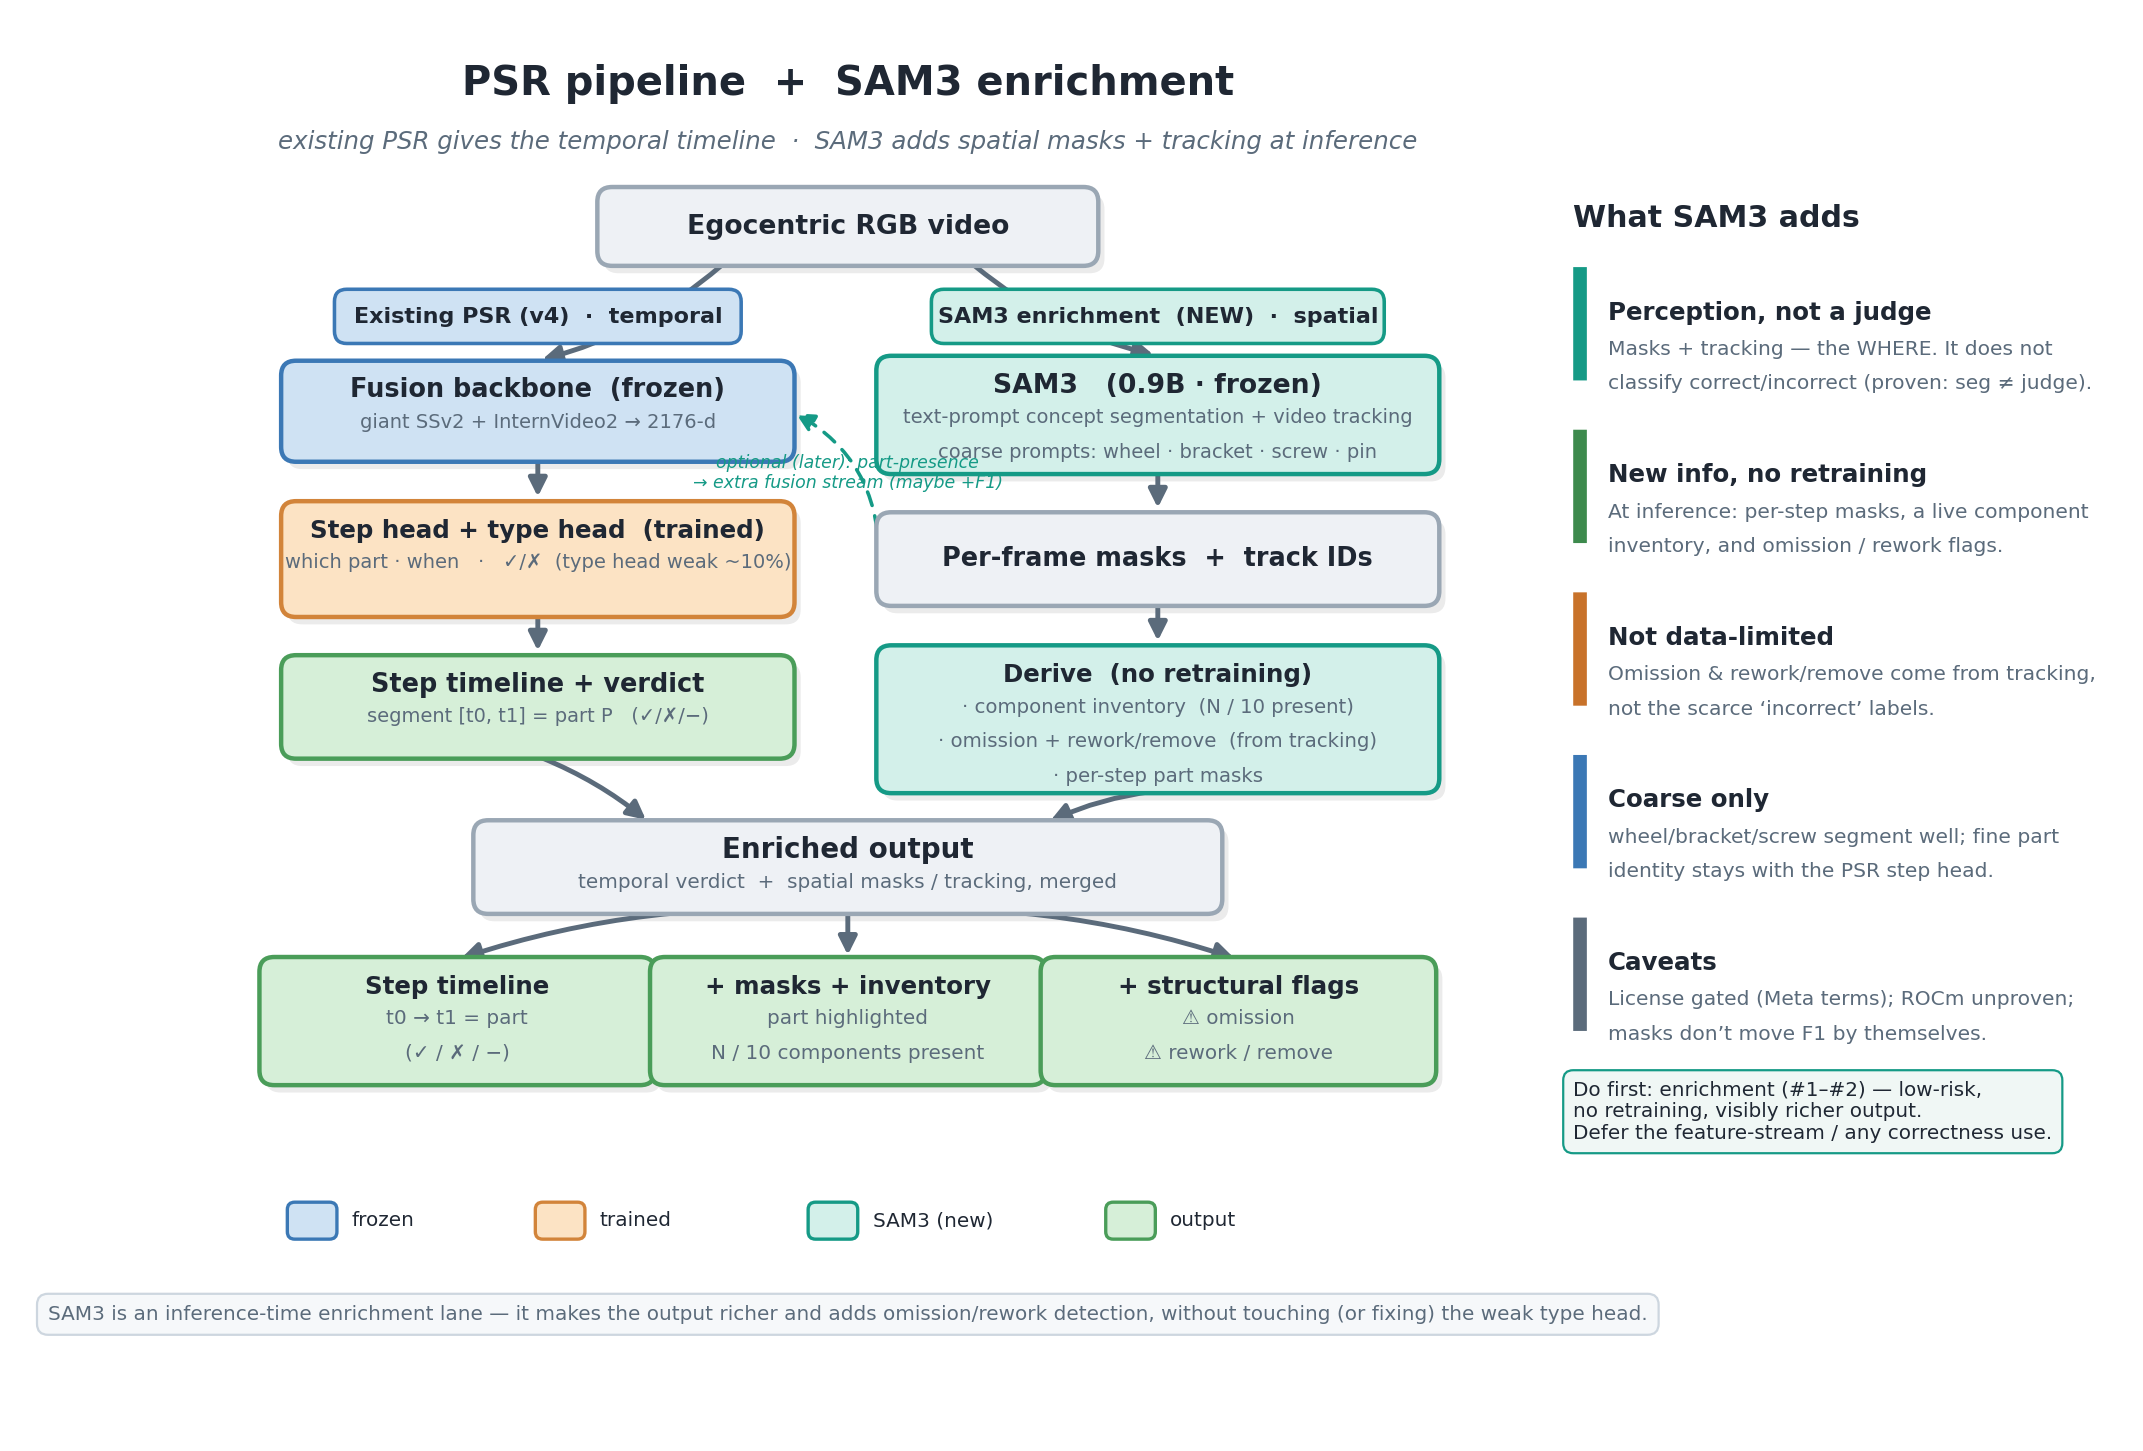
\includegraphics[width=0.98\linewidth]{architecture_sam3.png}
\caption{The v4 pipeline (temporal: which/when) with an added SAM3 enrichment lane (spatial: masks $+$ inventory),
converging into an enriched output. SAM3 is an inference-time add-on and does not alter the model or its accuracy.}
\label{fig:sam3}
\end{figure}

\begin{figure}[H]
\centering
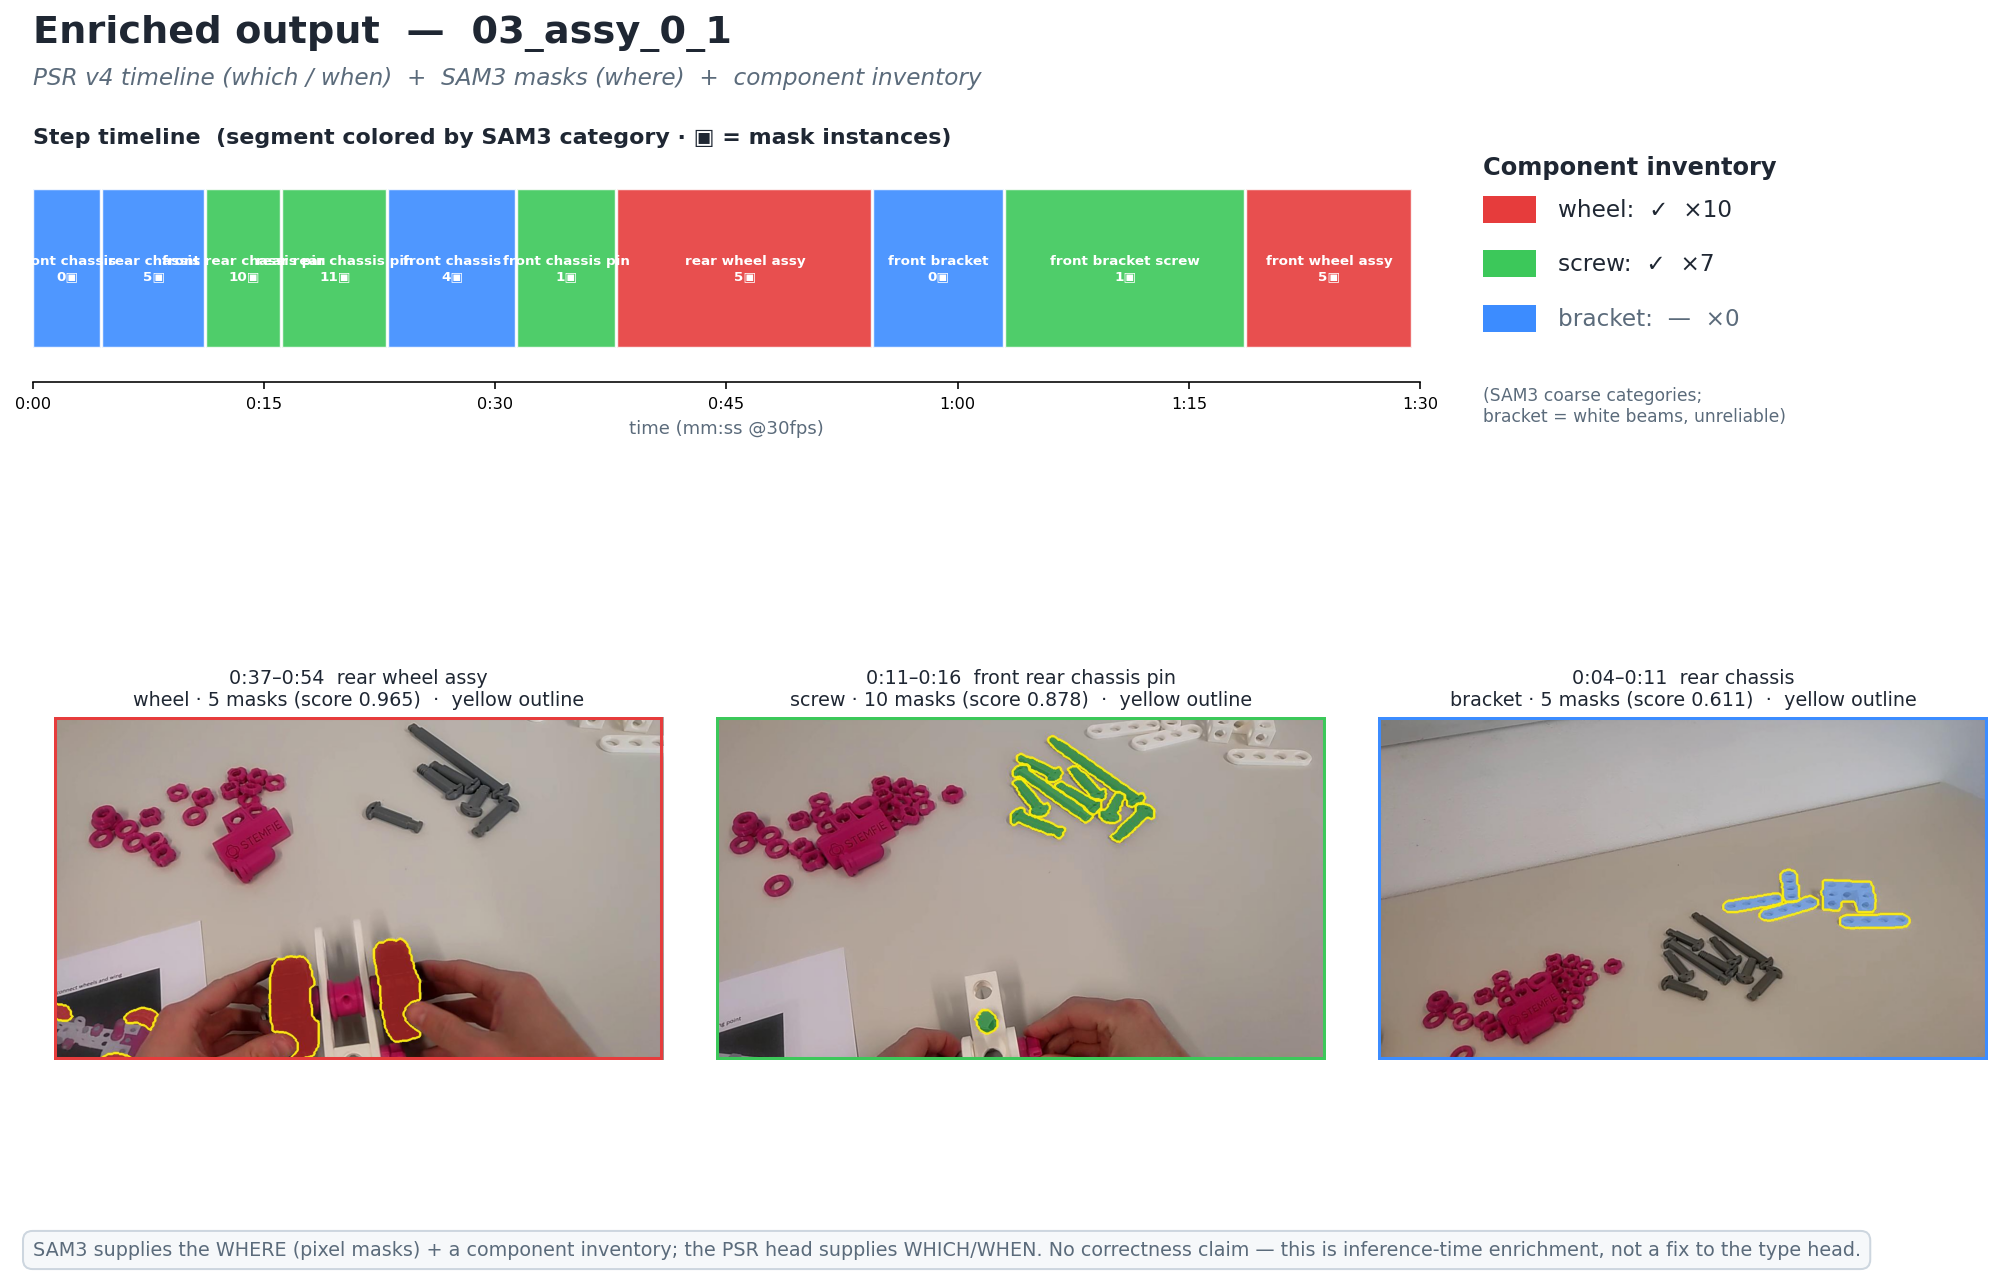
\includegraphics[width=0.98\linewidth]{enriched_output_panel.png}
\caption{Enriched output for one recording: the v4 step timeline (colored by SAM3 category), a component
inventory, and per-step SAM3 mask overlays (bright outlines). SAM3 supplies the \emph{where}; the v4 head supplies
the \emph{which/when}.}
\label{fig:enriched}
\end{figure}

\section{Results and Discussion}
Figure~\ref{fig:metrics} consolidates all comparisons. Three findings recur. (1) \textbf{Backbone $>$ head for
segmentation}: the SSv2-giant features help every head, and fusion helps further. (2) \textbf{The two wins are
orthogonal}: better features (fusion) and a better head (DiffAct) combine additively into v4. (3)
\textbf{Correctness is data-limited}: neither larger encoders nor foundation-model VLMs move it; the lever is more
error data and sharper labels. SAM3 enrichment is a pragmatic response---it makes the output visibly richer and
enables non-data-limited fault signals (omission, rework), while honestly not solving the wrong-install problem.

\begin{figure}[H]
\centering
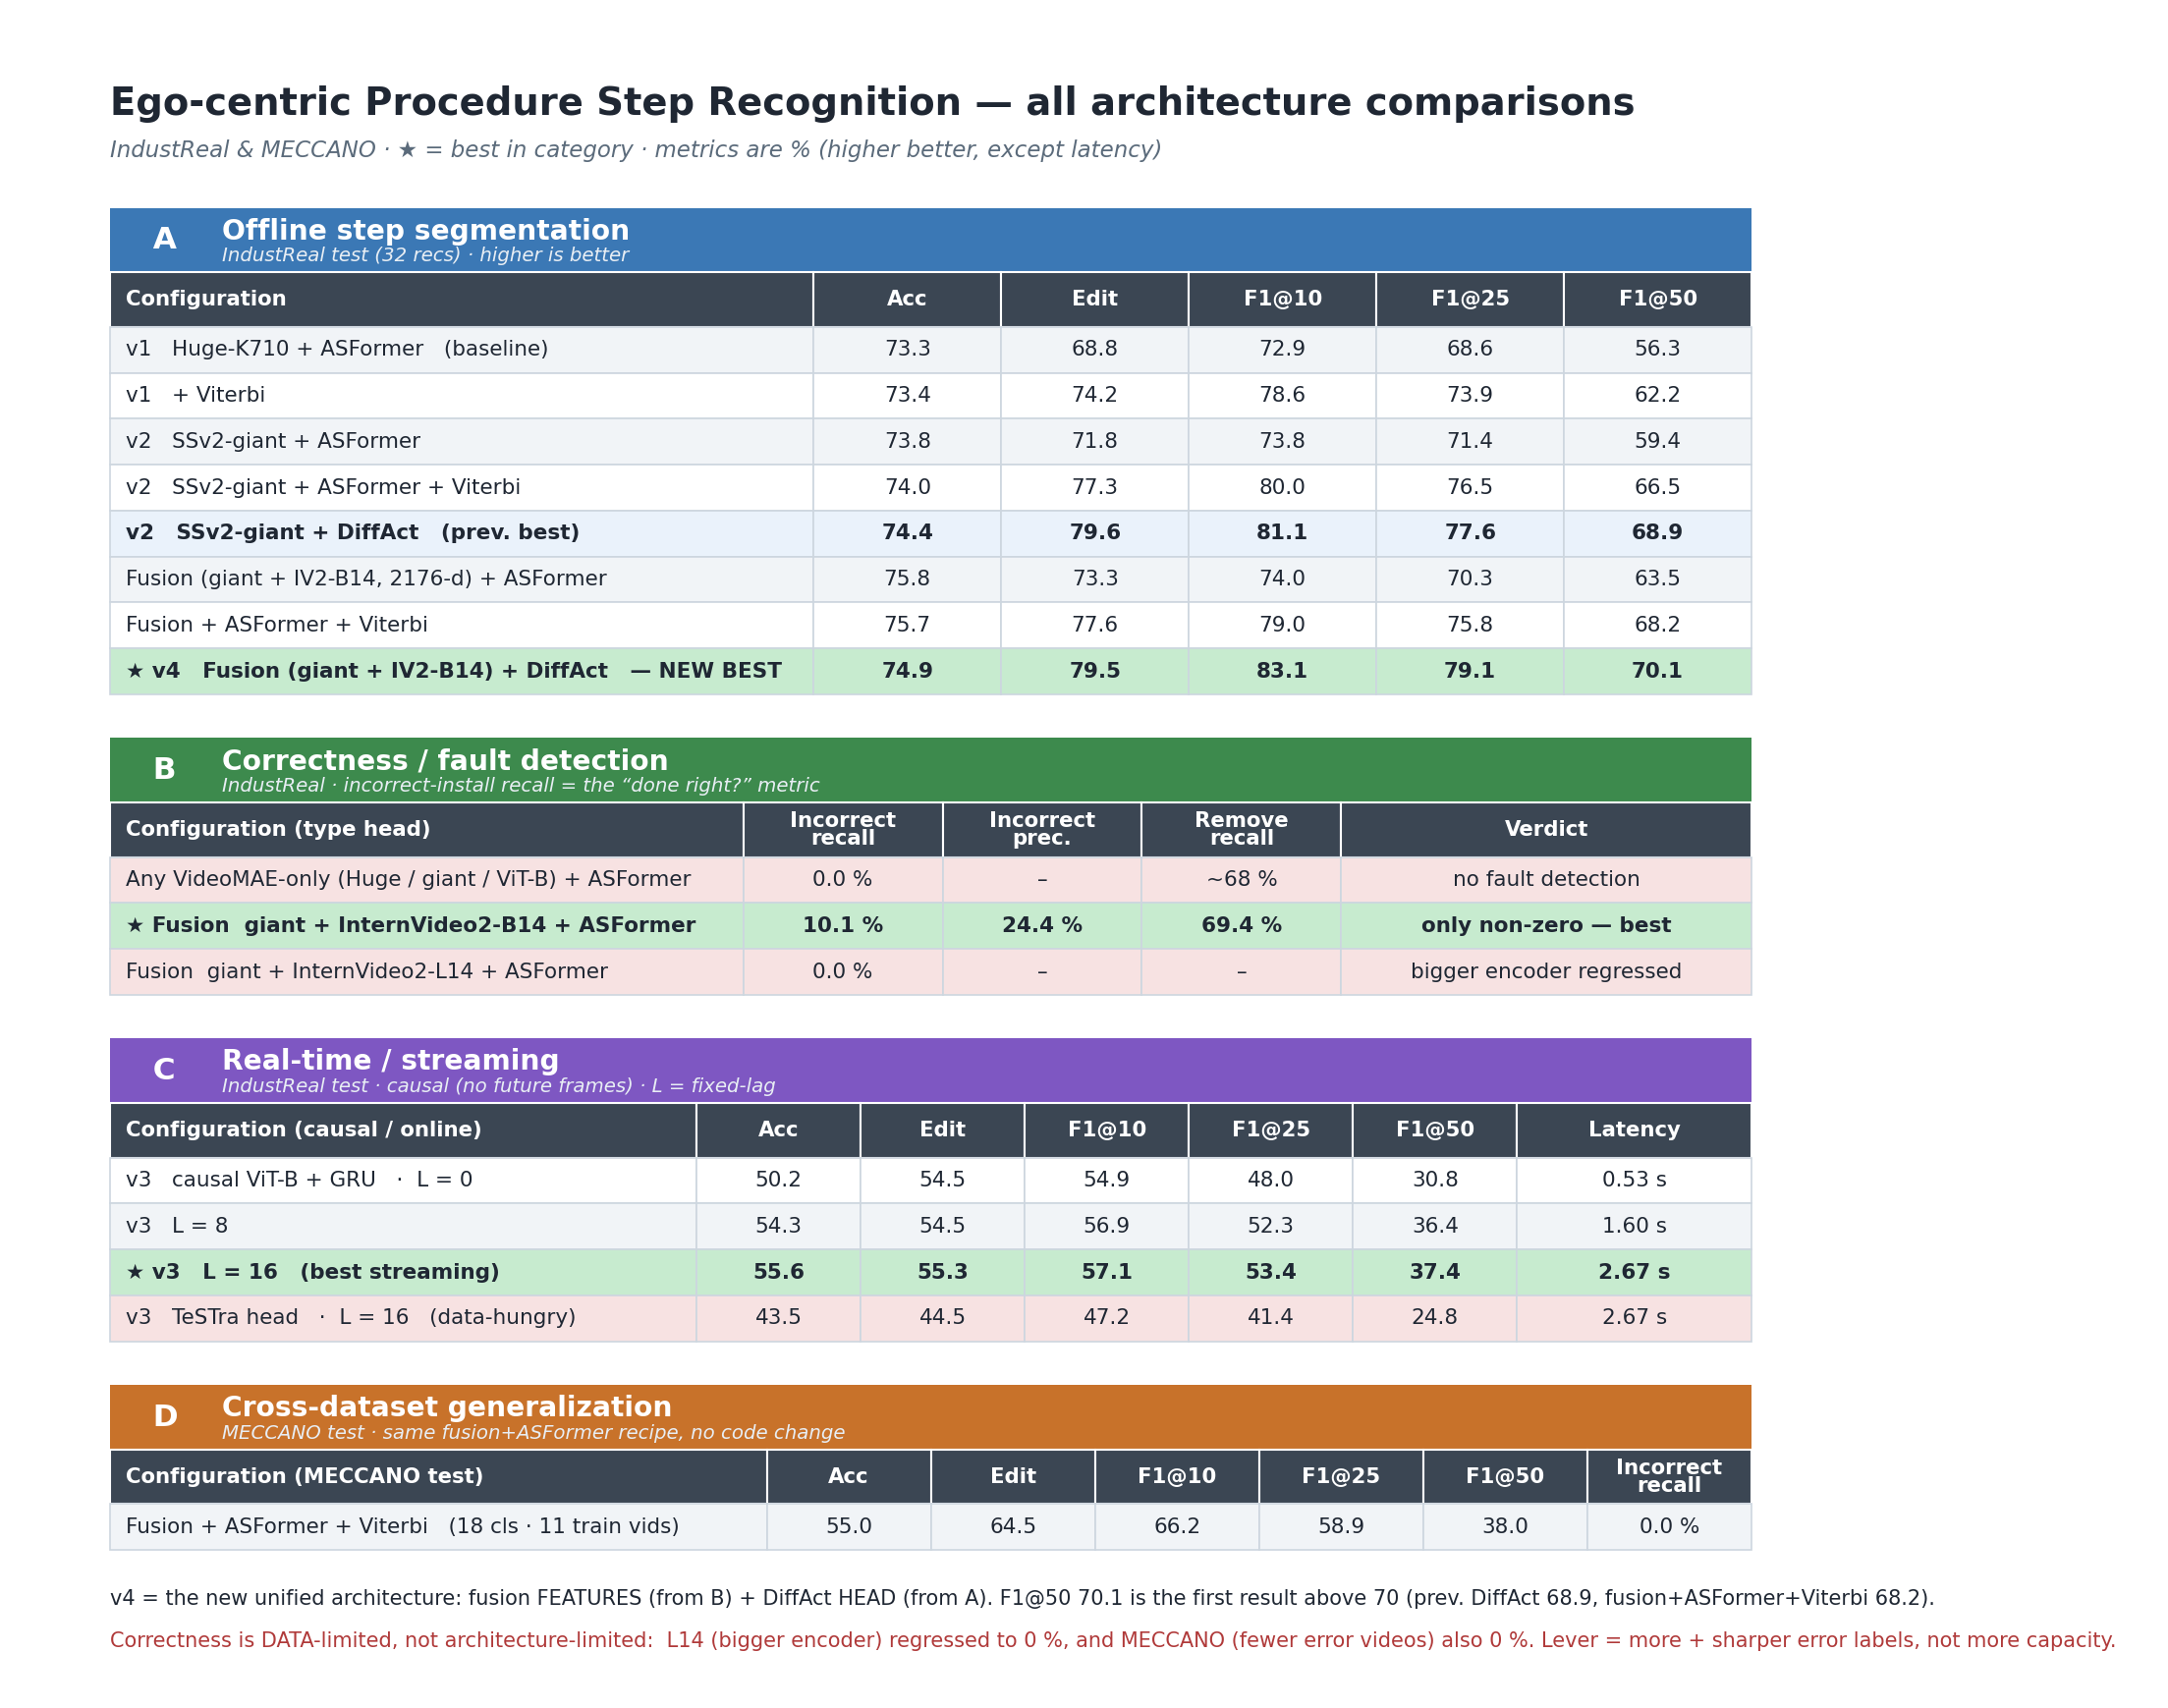
\includegraphics[width=0.96\linewidth]{metrics_comparison.png}
\caption{Consolidated comparison across all experiments: offline segmentation, fault detection, real-time
streaming, and cross-dataset generalization. Best-in-category rows are highlighted.}
\label{fig:metrics}
\end{figure}

\section{Conclusion}
We presented a controlled architecture progression for egocentric procedure step recognition in which each
change---Viterbi decoding, SSv2-giant features, the DiffAct head, and two-encoder fusion---improved segmentation,
ending at \best{v4 (Fusion $+$ DiffAct), F1@50 $=70.1$}. We built a causal real-time variant, confirmed
cross-dataset generalization, and characterized correctness as data-limited. Finally, we added a SAM3 enrichment
layer that augments the output with masks and a component inventory at no accuracy cost, and reported that
promptable foundation models localize but do not judge correctness. Future work targets the data-limited
correctness lever directly: sharper (segment-close) error labels, promotion of the non-data-limited \emph{remove}
class, and SAM3-based omission/rework detection against a reference bill-of-materials.

\begin{thebibliography}{99}
\small
\bibitem{industreal} T.~Schoonbeek \emph{et al.}, ``IndustReal: A Dataset for Procedure Step Recognition Handling
Execution Errors in Egocentric Videos,'' \emph{WACV}, 2024.
\bibitem{meccano} F.~Ragusa \emph{et al.}, ``The MECCANO Dataset: Understanding Human-Object Interactions from
Egocentric Videos in an Industrial-like Domain,'' \emph{WACV}, 2021.
\bibitem{mstcn} Y.~A.~Farha and J.~Gall, ``MS-TCN: Multi-Stage Temporal Convolutional Network for Action
Segmentation,'' \emph{CVPR}, 2019.
\bibitem{asformer} F.~Yi, H.~Wen, and T.~Jiang, ``ASFormer: Transformer for Action Segmentation,'' \emph{BMVC}, 2021.
\bibitem{diffact} D.~Liu \emph{et al.}, ``Diffusion Action Segmentation,'' \emph{ICCV}, 2023.
\bibitem{videomae} L.~Wang \emph{et al.}, ``VideoMAE V2: Scaling Video Masked Autoencoders with Dual Masking,''
\emph{CVPR}, 2023.
\bibitem{internvideo2} Y.~Wang \emph{et al.}, ``InternVideo2: Scaling Video Foundation Models for Multimodal Video
Understanding,'' \emph{ECCV}, 2024.
\bibitem{miniroad} S.~An \emph{et al.}, ``MiniROAD: Minimal RNN Framework for Online Action Detection,''
\emph{ICCV}, 2023.
\bibitem{testra} Y.~Zhao and P.~Kr\"ahenb\"uhl, ``Real-Time Online Video Detection with Temporal Smoothing
Transformers,'' \emph{ECCV}, 2022.
\bibitem{sam} A.~Kirillov \emph{et al.}, ``Segment Anything,'' \emph{ICCV}, 2023.
\bibitem{sam2} N.~Ravi \emph{et al.}, ``SAM 2: Segment Anything in Images and Videos,'' \emph{arXiv:2408.00714}, 2024.
\bibitem{sam3} Meta AI, ``SAM 3: Segment Anything with Concepts,'' Technical Report / \texttt{facebook/sam3}, 2025.
\bibitem{locateanything} NVIDIA, ``LocateAnything-3B: A Grounding Vision-Language Model,''
\texttt{nvidia/LocateAnything-3B}, 2025.
\bibitem{qwen25} Qwen Team, ``Qwen2.5 Technical Report,'' \emph{arXiv:2412.15115}, 2024.
\end{thebibliography}

\end{document}
